O controlador foi projetado com uma estrutura \gls{pd} paralela. Os ganhos
iniciais foram obtidos pelo método de Ziegler-Nichols a partir da
\Eqref{planta-sensor-1-zn} e posteriormente ajustados utilizando o \gls{rmse},
de acordo com a \Eqref{rmse}, como critério de desempenho.

\begin{equation}
  \eqlabel{rmse}
  \mathrm{RMSE} = \sqrt{\frac{1}{N}\sum_{k=1}^{N}{\left( r[k] - y[k] \right)}^{2}}
\end{equation}

O controlador \gls{pd} obtido é dado por \Eqref{controlador-pd-paralelo}.

\begin{equation}
  \eqlabel{controlador-pd-paralelo}
  C_{\mathrm{pd}}(s) = 13.472 + \frac{601.4s}{s+100}
\end{equation}

Apesar do bom desempenho dinâmico, o controlador \gls{pd} apresentou \gls{ess}
significativo durante o seguimento da referência.

Para reduzir esse erro, foi adicionada uma ação \gls{ff} baseada em um modelo
inverso da planta combinado com um filtro que define a dinâmica desejada em
malha fechada~\cite{astrom2021feedback,seborg2016process}.  Esse tipo de
controle utiliza o modelo do processo para antecipar a ação necessária ao
seguimento da referência~\cite{astrom2021feedback}.

Neste trabalho o \gls{ff} foi implementado com o modelo inverso da planta da
\Eqref{planta-sensor-1-zn} em paralelo com o \gls{pd}, além de um filtro
passa-baixas para garantir causalidade. O controlador resultante é dado por
\Eqref{controlador-ff}:

\begin{equation}
  \eqlabel{controlador-ff}
  C_{\mathrm{ff}} = \frac{188.0271s + 1}{6.075 s + 0.92}
\end{equation}

A \Figref{bloco-controlador} mostra a estrutura completa do controlador. Nela, o
\gls{ff} atua diretamente sobre a referência, enquanto o \gls{pd} corrige o erro
pela realimentação do sistema.

\begin{figure}[H]
\centering
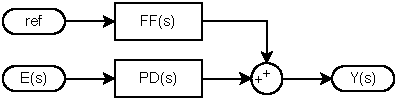
\includegraphics[width=1\linewidth]{images/Bloco Controlador.pdf}
\caption{Estrutura do controlador proposto, composta por uma ação \gls{ff}
aplicada à referência e uma ação \gls{pd} baseada na realimentação do sistema.}
\figlabel{bloco-controlador}
\end{figure}

O controlador foi discretizado pelo método de Tustin, aplicado às ações \gls{pd}
e \gls{ff}. Nesse método, o operador contínuo $s$ é aproximado pela
transformação bilinear conforme a \Eqref{tustin}.

\begin{equation}
  \eqlabel{tustin}
  s \approx \frac{2}{T_s}\frac{z-1}{z+1},
\end{equation}

Onde $T_s$ é o período de amostragem definido como $T_s = \SI{15}{\second}$.
O modelo da planta foi discretizado por \gls{zoh}, resultando na
\Eqref{planta-gz-zoh}.

\begin{equation}
  \eqlabel{planta-gz-zoh}
  G(z) = z^{-1} \cdot \frac{0.0413z + 0.0293}{z - 0.9233}
\end{equation}

